\documentclass[11pt]{article} % use larger type; default would be 10pt

\usepackage{float}
\usepackage[utf8]{inputenc} % set input encoding (not needed with XeLaTeX)
\usepackage{adjustbox}   
%%% Examples of Article customizations
% These packages are optional, depending whether you want the features they provide.
% See the LaTeX Companion or other references for full information.
  
%%%%%%%%%%%%%%%%%%%%%%%%%%formatting cells colors
\usepackage[table,x11names,dvipsnames]{xcolor}
 \usepackage{collcell}
 \usepackage{array}
 \usepackage{tikz}
 \usepackage{relsize}
  \usepackage{pgfkeys}
 \usepackage{graphicx}
 \usepackage{xspace}
 \usepackage{amsmath,amssymb}

%%% PAGE DIMENSIONS
\usepackage{geometry} % to change the page dimensions
\geometry{a4paper} % or letterpaper (US) or a5paper or....
 \geometry{margin=1in} % for example, change the margins to 2 inches all round
% \geometry{landscape} % set up the page for landscape
%   read geometry.pdf for detailed page layout information
\usepackage{multicol}
\usepackage{booktabs}
\usepackage{todonotes}
\usepackage{times}
\usepackage{inconsolata}

\usepackage[figurename=Supplementary~Figure, tablename=Supplementary~Table]{caption}
\DeclareCaptionLabelFormat{cont}{Figure S\arabic{figure}}
\captionsetup[figure]{labelformat=cont}
\DeclareCaptionLabelFormat{contt}{Table S\arabic{table}}
\captionsetup[table]{labelformat=contt}
\captionsetup{labelfont={bf}}

%%%%%% TIKZ %%%%%%%%%%%%%%%%%%%%%%%%

\tikzstyle{startend}=[rectangle, rounded corners, minimum width=2cm,  minimum height=1cm, text width =2cm, text centered, draw=none, fill= orange!50, font=\sf]
\tikzstyle{io}=[trapezium, trapezium left angle=70,trapezium right angle= 110,minimum width=3.9cm, minimum height=1cm, text centered, draw=none, fill= blue!30, font=\sf]

\tikzstyle{process}=[rectangle, minimum width=3cm,maximum width=3, minimum height=1cm, text centered, draw=black, fill= orange!30, font=\sffamily]
\tikzstyle{Vprocess}=[rectangle, minimum width=6cm, minimum height=1cm, text centered, font=\sf\bfseries,  fill= gray!80, draw=none, text=white]
\tikzstyle{VSprocess}=[rectangle, minimum width=1cm, minimum height=2cm, text centered, font=\sf\bfseries,  fill= gray!80, draw=none, text=white]
\tikzstyle{squareprocess}=[rectangle, minimum width=2cm, minimum height=7cm, text centered, draw=black, fill= orange!30, font=\sffamily]
\tikzstyle{Bprocess}=[rectangle, minimum width=6cm, minimum height=1cm, text centered,  font=\sf\bfseries,  fill= cyan!60!black, draw=none, text=white]
\tikzstyle{BSprocess}=[rectangle, minimum width=3cm, minimum height=1cm, text centered, draw=black, fill= orange!30, font=\sffamily]
\tikzstyle{decision}=[diamond, minimum width=2.5cm, minimum height=1.5cm, align=center, inner sep=-5pt ,font=\sf\bfseries,  fill= PineGreen!60, draw=none, text=white]
\tikzstyle{IO}=[text=white]

\tikzstyle{arrow}=[line width=1.5pt, ->, >=stealth, gray!80!black]
\tikzstyle{arrowcaption}=[font=\sf\relsize{+1},black]
\tikzstyle{input}=[fill= gray!80!black, inner sep=5pt,rounded corners=5pt]
\tikzstyle{output}=[fill= gray!80!black, inner sep=5pt,rounded corners=5pt]

\pgfkeys{/heat/.is family, /heat,
	Max colour/.initial = Green4,
	Min colour/.initial = Red1,
	max colour/.initial = SpringGreen3,
	mid colour/.initial = white,
	min colour/.initial = Yellow1,
	text colour/.initial = black,
	Min color/.style = {Min colour=#1},% for our friends who can't spell
	Max color/.style = {Max colour=#1},
	min color/.style = {min colour=#1},
	mid color/.style = {mid colour=#1},
	max color/.style = {max colour=#1},
	text color/.style = {text colour=#1},
	min/.initial = -1,
	mid/.initial = 0,
	max/.initial = 1,
	slider/.code={%
		\tikz{\shade[left color=\HVal{min colour},%
			right color=\HVal{max colour}]%
			(current page.south west) rectangle ++(#1,12pt);
		}%
	}%
}

\newcommand{\tikzcircle}[2][red,fill=red]{\tikz[baseline=-0.5ex]\draw[#1,radius=#2] (0,0) circle ;}%
\newcommand\Heatset[1]{\pgfkeys{/heat, #1}}
\newcommand\HVal[1]{\pgfkeysvalueof{/heat/#1}}

\newcolumntype{H}{>{\collectcell\Heat}r<{\endcollectcell}}
\newcommand\Heat[1]{% \Heat{number in the interval [min, max] }
	\if\relax\detokenize{#1}\relax% empty cell
	\else%
	\pgfmathparse{int(100*(#1-\HVal{min})/(\HVal{max}-\HVal{min}))}% map number to [0,100]
	\ifnum\pgfmathresult>100% too big
	\edef\HeatCell{\noexpand\cellcolor{\HVal{Max colour}}}%
	\else\ifnum\pgfmathresult<0% too small
	\edef\HeatCell{\noexpand\cellcolor{\HVal{Min colour}}}%
	\else\ifnum\pgfmathresult<50% between min and mid
	\pgfmathparse{int(2*\pgfmathresult)}% map number to [0,100]
	\edef\HeatCell{\noexpand\cellcolor{\HVal{mid colour}!\pgfmathresult!\HVal{min colour}}}%
	\else% between min and max
	\pgfmathparse{int(2*(\pgfmathresult-50))}% map number to [0,100]
	\edef\HeatCell{\noexpand\cellcolor{\HVal{max colour}!\pgfmathresult!\HVal{mid colour}}}%
	\fi%
	\fi%
	\fi%
	\HeatCell\textcolor{\HVal{text colour}}{$#1$}%
	\fi%
}

\pgfkeys{/heatsec/.is family, /heatsec,
	Max colour/.initial = Green4,
	Min colour/.initial = Red1,
	max colour/.initial = SpringGreen3,
	mid colour/.initial = white,
	min colour/.initial = Yellow1,
	text colour/.initial = black,
	Min color/.style = {Min colour=#1},% for our friends who can't spell
	Max color/.style = {Max colour=#1},
	min color/.style = {min colour=#1},
	mid color/.style = {mid colour=#1},
	max color/.style = {max colour=#1},
	text color/.style = {text colour=#1},
	min/.initial = -1,
	mid/.initial = 0,
	max/.initial = 1,
	slider/.code={%
		\tikz{\shade[left color=\HVal{min colour},%
			right color=\HVal{max colour}]%
			(current page.south west) rectangle ++(#1,12pt);
		}%
	}%
}
\newcommand\HeatSecset[1]{\pgfkeys{/heatsec, #1}}
\newcommand\HSVal[1]{\pgfkeysvalueof{/heatsec/#1}}

\colorlet{BadCol}{Burlywood1!70!red}


\newcolumntype{S}{>{\collectcell\HeatSec}r<{\endcollectcell}}
\newcommand\HeatSec[1]{% \Heat{number in the interval [min, max] }
	\if\relax\detokenize{#1}\relax% empty cell
	\else%
	\pgfmathparse{int(100*(#1-\HSVal{min})/(\HSVal{max}-\HSVal{min}))}% map number to [0,100]
	\ifnum\pgfmathresult>100% too big
	\edef\HeatCell{\noexpand\cellcolor{\HSVal{Max colour}}}%
	\else\ifnum\pgfmathresult<0% too small
	\edef\HeatCell{\noexpand\cellcolor{\HSVal{Min colour}}}%
	\else\ifnum\pgfmathresult<50% between min and mid
	\pgfmathparse{int(2*\pgfmathresult)}% map number to [0,100]
	\edef\HeatCell{\noexpand\cellcolor{\HSVal{mid colour}!\pgfmathresult!\HSVal{min colour}}}%
	\else% between min and max
	\pgfmathparse{int(2*(\pgfmathresult-50))}% map number to [0,100]
	\edef\HeatCell{\noexpand\cellcolor{\HSVal{max colour}!\pgfmathresult!\HSVal{mid colour}}}%
	\fi%
	\fi%
	\fi%
	\HeatCell\textcolor{\HSVal{text colour}}{$#1$}%
	\fi%
}

%%%%%% MACROS %%%%%%%%%%%%%%%%%%%%%%%%

\definecolor{lightsalmon}{rgb}{1.0, 0.63, 0.48}
\definecolor{lightseagreen}{rgb}{0.13, 0.7, 0.67}
\definecolor{americanrose}{rgb}{1.0, 0.01, 0.24}
\DeclareMathOperator*{\argmin}{\arg\!\min}
\DeclareMathOperator*{\argmax}{\arg\!\max}
\newcommand{\multicoomment}[1]{}
\newcommand{\Software}[1]{\text{\ttfamily\bfseries #1}}
\newcommand{\OurTool}{\Software{IPANEMAP}\xspace}
\newcommand{\SM }{{\tt SHAPEMap}\xspace}
\newcommand{\SH }{{\tt SHAPE}\xspace}
\newcommand{\VP }{{\tt Vienna package}\xspace}
\newcommand{\OurRna}{\Software{Did}\xspace}
\newcommand{\mm }{{\tt$M\&M$}\xspace}
\newcommand{\DP }{{\tt DP}\xspace}
\newcommand{\didy }{{\sf GIR1 Lariat-capping ribozyme}\xspace}

\newcommand{\CE }{{\tt capillary electrophoresis}\xspace}
%MPCRnas MultiProbing Conformers}}
% Macros for # variables
\newcommand{\BP }{{\mathcal{ BP}}}
\newcommand{\Ensemble }{{\mathcal{ S}}}
\newcommand{\Sample }{{\mathcal{ S_D}}}
\newcommand{\PData }[1]{{\mathcal{ D}_{#1}}}
\newcommand{\Bzcond}[1]{ \mathbb{P}(s\mid #1)}
\newcommand{\CBP}[1]{ \mathbb{CP}_#1}
\newcommand{\BF}{ \mathbb{BF}}
\newcommand{\Zed}{\mathbb{Z}}
\newcommand{\Edist }{{ \text{Dist}}}
\newcommand{\RL }{{n}}
\newcommand{\CL}{MBkM\xspace}
\newcommand{\Clusters}{\mathcal{C}}
\newcommand{\Centroids}{\mathcal{C_O}}
\newcommand{\GMean}{\text{GM}}
\newcommand{\Ref}{R}
%\newcommand{\OurRna}{\Software{Did}}
%MPCRnas MultiProbing Conformers}}
\newcommand{\NumClust}{k}
\newcommand{\etal}{~\emph{et al} }
\newcommand{\Def}[1]{{\em #1}}

%%% Conditions
\newcommand{\Cond}[5]{\textsc{#1-#3$^{\text{#2}}_{\text{#4}}$#5}}

\newcommand{\OneMSevILUMg}{\Cond{1M7}{mg}{MaP}{il}{}\xspace}
\newcommand{\OneMSevILU}{\Cond{1M7}{}{MaP}{il}{}\xspace}

\newcommand{\OneMSevILUThreeMg}{\Cond{1M7}{mg}{MaP}{il}{-3d}\xspace}
\newcommand{\OneMSevILUThree}{\Cond{1M7}{}{MaP}{il}{-3d}\xspace}

\newcommand{\OneMSevMgCE}{\Cond{1M7}{mg}{CE}{}{}\xspace}
\newcommand{\OneMSevCE}{\Cond{1M7}{}{CE}{}{}\xspace}

\newcommand{\CMCTMg}{\Cond{CMCT}{mg}{CE}{}{}\xspace}

\newcommand{\NMIA}{\Cond{NMIA}{}{MaP}{it}{}\xspace}
\newcommand{\NMIAMg}{\Cond{NMIA}{mg}{MaP}{it}{}\xspace}

\newcommand{\NMIACE}{\Cond{NMIA}{}{CE}{}{}\xspace}
\newcommand{\NMIAMgCE}{\Cond{NMIA}{mg}{CE}{}{}\xspace}

\newcommand{\NAIMg}{\Cond{NAI}{mg}{CE}{}{}\xspace}
\newcommand{\NAICE}{\Cond{NAI}{}{CE}{}{}\xspace}

\newcommand{\BzCN}{\Cond{BzCN}{}{CE}{}{}\xspace}
\newcommand{\BzCNMg}{\Cond{BzCN}{mg}{CE}{}{}\xspace}

\newcommand{\DMSMg}{\Cond{DMS}{mg}{CE}{}{}\xspace}

\newcommand{\BZCNCE}{\Cond{BzCN}{}{CE}{}{}\xspace}


\newcommand{\Draft}[1]{{#1}}
\newcommand{\bs}[1]{\Draft{\todo[color=red!30]{\sf Bruno: #1}}}
\newcommand{\bsi}[1]{\Draft{\todo[color=red!30,inline]{\sf Bruno: #1}}}
\newcommand{\as}[1]{\Draft{\todo[color=green!70!black]{\sf Afaf: #1}}}
\newcommand{\yp}[1]{\Draft{\todo[color=blue!30]{\sf Yann: #1}}}
\newcommand{\ypi}[1]{\Draft{\todo[color=blue!30,inline]{\sf Yann: #1}}}

%\renewcommand{\bsi}[1]{}
%\renewcommand{\ypi}[1]{}

\newcommand{\ipanemapurl}{https://github.com/afafbioinfo/IPANEMAP}

\newcommand{\Bull}[1]{{\sffamily #1}~\raisebox{1pt}{\tikzcircle[black, fill=cluster#1]{3pt}}}

\newcommand{\BullLab}[1]{Cluster \Bull{#1}}

\colorlet{clusterA}{SeaGreen}
\colorlet{clusterB}{Yellow}
\colorlet{clusterC}{gray}
\definecolor{clusterD}{HTML}{AFAFE9}
\colorlet{clusterE}{OliveGreen}
\colorlet{clusterF}{blue!90!black}
\colorlet{clusterG}{Orange}
\colorlet{clusterH}{SeaGreen!40}




\title{\OurTool{}:  Integrative Probing Analysis of Nucleic Acids Empowered by Multiple Accessibility Profiles\\[1em]
	Supplementary material
}
\author{}
\date{} % Activate to display a given date or no date (if empty),
         % otherwise the current date is printed 
\newcommand{\Start}{s}
\newcommand{\End}{e}


\begin{document}
\maketitle

\tableofcontents

\section{Multiprobing benchmark (Cordero~\emph{et al}~\cite{Cordero2012} dataset)}
\subsection{MCC values of individual predictions}

 \Heatset{min=0.4,  
	max=1,   
	max colour=Aquamarine3, % colour at maximum
	min colour=BadCol,      % colour at minimum
	Min colour=BadCol, % colour for values below min
	Max colour=Aquamarine3   % colour for values above max
}

\begin{table}[H]
\centering
\newcommand{\B}{\multicolumn{1}{c}{$\bullet$}}
\newcommand{\BR}{\multicolumn{1}{c}{$\bullet$}}
\newcommand{\D}{\multicolumn{1}{c}{\color{gray}$\circ$}}
\newcommand{\DR}{\multicolumn{1}{c}{\color{gray}$\circ$}}
\begin{adjustbox}{max width=1\textwidth}
 \begin{tabular}{@{}lHHHHHHHHHHHHHHHH@{}}
 	\toprule
 	                              & \multicolumn{8}{l}{ \OurTool{}}                                     & \multicolumn{4}{l}{\Software{RNAfold} -- MFE mode} & \multicolumn{4}{l}{\Software{RNAfold} -- MEA mode}  \\
 	\textbf{CMCT}                 & \D    & \B    & \D       & \D    & \D    & \B       & \B    & \BR   & \D       & \D    & \B    & \DR                     & \D    & \D    & \B       & \D                       \\
 	\textbf{NMIA}                 & \D    & \D    & \B       & \D    & \B    & \D       & \B    & \BR   & \D       & \D    & \D    & \BR                     & \D    & \D    & \D       & \B                       \\
 	\textbf{DMS}                  & \D    & \D    & \D       & \B    & \B    & \B       & \D    & \BR   & \D       & \B    & \D    & \DR                     & \D    & \B    & \D       & \D                       \\ \midrule
 	5SRNA,E.Coli                  & 0.25  & 0.238 & 0.247    & 0.244 & 0.247 & 0.247    & 0.254 & 0.241 & 0.241    & 0.686 & 0.254 & 0.686                   & 0.241 & 0.686 & 0.269    & 0.686                    \\
 	glycineriboswitch,F.nucleatum & 0.568 & 0.627 & 0.868    & 0.952 & 0.868 & 0.658    & 0.868 & 0.868 & 0.306    & 0.313 & 0.395 & 0.313                   & 0.593 & 0.593 & 0.693    & 0.6                      \\
 	cidGMPriboswitch,V.Cholerae   & 0.654 & 0.77  & 0.654    & 0.77  & 0.654 & 0.77     & 0.654 & 0.77  & 0.77     & 0.77  & 0.667 & 0.77                    & 0.77  & 0.72  & 0.667    & 0.77                     \\
 	P4P6domain                    & 0.864 & 0.856 & 0.881    & 0.864 & 0.864 & 0.856    & 0.864 & 0.856 & 0.837    & 0.808 & 0.773 & 0.714                   & 0.845 & 0.808 & 0.781    & 0.722                    \\
 	adenineriboswitch,add         & 1     & 0.956 & 1        & 0.977 & 1     & 0.956    & 1     & 1     & 1        & 0.333 & 0.41  & 1                       & 1     & 0.333 & 0.356    & 0.306                    \\
 	tRNAphenylalanineyeast        & 0.286 & 0.746 & 0.976    & 0.746 & 0.976 & 0.746    & 0.976 & 0.976 & 0.976    & 0.976 & 0.976 & 0.976                   & 0.334 & 0.976 & 0.976    & 0.976                    \\ \midrule
 	Average                       & 0.604 & 0.7   & 0.77     & 0.76  & 0.77  & 0.705    & 0.77  & 0.785 & 0.69     & 0.65  & 0.58  & 0.74                    & 0.63  & 0.69  & 0.62     & 0.68                     \\ \bottomrule
 \end{tabular}
\end{adjustbox}
\caption{GM of the structures predicted with \OurTool{}, compared to predictions of \Software{RNAfold} in energy mimization (MFE) and accuracy maximization (MEA) modes.}
%( ref. $supplementary\_data/benchmark\_6RNAs$)}
\end{table}
\subsection{Stablity analysis}
\begin{table}[H]
\centering
\begin{adjustbox}{max width=1\textwidth}
 \begin{tabular}{lHHHHHHHHHHHHHHHHHHHHH}\toprule
 &\multicolumn{3}{l}{ NMIA} & \multicolumn{3}{l}{ DMS} & \multicolumn{3}{l}{CMCT} &\multicolumn{3}{l}{ NMIA+DMS} & \multicolumn{3}{l}{ NMIA+CMCT} & \multicolumn{3}{l}{DMS+CMCT}& \multicolumn{3}{l}{NMIA+DMS+CMCT} \\
% & \multicolumn{3}{l}{ GM }  & \multicolumn{3}{l}{ GM } & \multicolumn{3}{l}{ GM }& \multicolumn{3}{l}{ GM }  & \multicolumn{3}{l}{ GM } & \multicolumn{3}{l}{ GM } &\multicolumn{3}{l}{ GM }\\

Replicates& \multicolumn{1}{l}{Run 1} & \multicolumn{1}{l}{Run 2} & \multicolumn{1}{l}{Run 3} & \multicolumn{1}{l}{Run 1} & \multicolumn{1}{l}{Run 2} & \multicolumn{1}{l}{Run 3}& \multicolumn{1}{l}{Run 1} & \multicolumn{1}{l}{Run 2} & \multicolumn{1}{l}{Run 3} & \multicolumn{1}{l}{Run 1} & \multicolumn{1}{l}{Run 2} & \multicolumn{1}{l}{Run 3}& \multicolumn{1}{l}{Run 1} & \multicolumn{1}{l}{Run 2} & \multicolumn{1}{l}{Run 3} & \multicolumn{1}{l}{Run 1} & \multicolumn{1}{l}{Run 2} & \multicolumn{1}{l}{Run 3}& \multicolumn{1}{l}{Run 1} & \multicolumn{1}{l}{Run 2} & \multicolumn{1}{l}{Run 3}\\
\midrule
5SRNA,E.Coli	&	0.247	&	0.25	&	0.247	&	0.254	&	0.244	&	0.244	&	0.238	&	0.238	&	0.238	&	0.247	&	0.244	&	0.247	&	0.257	&	0.238	&	0.238	&	0.247	&	0.247	&	0.244	&	0.241	&	0.241	&	0.241	\\
glycineriboswitch,F.nucleatum	&	0.868	&	0.868	&	0.868	&	0.952	&	0.952	&	0.952	&	0.868	&	0.634	&	0.627	&	0.868	&	0.868	&	0.868	&	0.868	&	0.868	&	0.868	&	0.667	&	0.658	&	0.658	&	0.868	&	0.868	&	0.868	\\
cidGMPriboswitch,V.Cholerae	&	0.631	&	0.631	&	0.631	&	0.77	&	0.77	&	0.77	&	0.667	&	0.77	&	0.77	&	0.631	&	0.631	&	0.756	&	0.77	&	0.77	&	0.77	&	0.77	&	0.77	&	0.77	&	0.77	&	0.77	&	0.77	\\
P4P6domain	&	0.864	&	0.881	&	0.881	&	0.864	&	0.864	&	0.856	&	0.856	&	0.856	&	0.856	&	0.864	&	0.864	&	0.864	&	0.864	&	0.864	&	0.864	&	0.856	&	0.856	&	0.856	&	0.856	&	0.856	&	0.856	\\
adenineriboswitch,ad	&	1	&	1	&	1	&	0.956	&	0.956	&	0.956	&	1	&	0.956	&	0.956	&	1	&	1	&	1	&	1	&	1	&	1	&	0.956	&	0.956	&	0.956	&	1	&	1	&	1	\\
tRNAphenylalanineyeast	&	0.953	&	0.953	&	0.976	&	0.976	&	0.746	&	0.976	&	0.746	&	0.746	&	0.746	&	0.976	&	0.976	&	0.976	&	0.976	&	0.976	&	0.97	&	0.746	&	0.746	&	0.746	&	0.746	&	0.976	&	0.976	\\

\bottomrule
\end{tabular}
\end{adjustbox}
\caption{GM of \OurTool predictions over three consecutive runs from up 3 sources of probing data.}
%( ref. $supplementary\_data/benchmark\_6RNAs$)
\end{table}


%\section{IPANEMAP Vs Rsample}
\section{Mono probing benchmark (Hajdin~\emph{et al}~\cite{Hajdin2013} dataset)}

 \begin{table}[H]
{\centering
\begin{adjustbox}{max width=1\textwidth}
 \begin{tabular}{@{}llll@{}}
 	\toprule
 	RNA ID & Description                      \\ \midrule
 	A      & Pre-Q1 riboswitch, B. subtilis      & 	M      &SARS corona virus pseudoknot       \\
 	B      & 5’ domain of 16S rRNA, E. coli            & 	N      & 	5S rRNA, E. coli                      \\
 	C      &	Signal recogniton particle RNA human & 	O      & cyclic-di-GMP riboswitch, V. cholerae   \\
 	D      & 	Group I intron, Azoarcus sp.          & 	P      & 5’ domain of 23S rRNA, E. coli            \\
 	E      & 	HIV 15 prime pseudoknot domain       & 	Q      & RNase PB. subtilis                \\
 	F      & Telomerase pseudoknot human       & 	R      & 	Group I Intron, T. thermophila        \\
 	G      & 	SAM I riboswitch, T. tengcongensis   & 	S      & 	Hepatitis C virus IRES domain       \\
 	H      & 	tRNA(phe), E. coli                & 	T      & 	5' domain of 16S rRNA, H. volcanii      \\
 	I      & P546 domain, bI3 group I intron       & 	U      & 	Group II intron, O. iheyensis         \\
 	J      & TPP riboswitch, E. coli              & 	V      & 	tRNA(asp), yeast                    \\
 	K      &	Adenine riboswitch, V. vulnificus    & 	W      & 	Lysine riboswitch, T. maritima        \\
 	L      & Fluoride riboswitch, P. syringae     & 	X      & M-Box riboswitch, B. subtilis          \\
 	\bottomrule
 \end{tabular}
\end{adjustbox}\\}

\caption{Labels used as shorthands for the 24 RNAs in the Hajdin \emph{ et al.} dataset~\cite{Hajdin2013}.}
\label{clyu}

\end{table}

\subsection{Detailed results of \OurTool{} and \Software{Rsample}}
\begin{table}[H]
	{\centering \begin{adjustbox}{max width=\textwidth,max totalheight=\textheight,keepaspectratio}
			\begin{tabular}{llllHllH}
				\toprule
				&        & \multicolumn{3}{l}{\Software{Rsample}}    & \multicolumn{3}{l}{\Software{IPANEMAP}}   \\
				{RNA} & Length & Sensitivity & PPV    & \multicolumn1c{GM} & Sensitivity & PPV    & \multicolumn1c{GM} \\ \midrule
				A     & 34     & 0.625       & 1      & 0.791              & 0.625       & 1      & 0.791              \\
				B     & 530    & 0.6622      & 0.6203 & 0.641              & 0.8986      & 0.8062 & 0.851              \\
				C     & 301    & 0.03        & 0.0313 & 0.031              & 0.6         & 0.6    & 0.6                \\
				D     & 214    & 0.6349      & 0.6667 & 0.651              & 0.7302      & 0.8519 & 0.789              \\
				E     & 500    & 0.6382      & 0.7823 & 0.707              & 0.5263      & 0.5517 & 0.539              \\
				F     & 47     & 0.4         & 0.75   & 0.548              & 0.6         & 0.75   & 0.671              \\
				G     & 118    & 0.7179      & 0.8    & 0.758              & 0.7692      & 0.8333 & 0.801              \\
				H     & 76     & 0.4762      & 0.5556 & 0.514              & 0.7619      & 0.7619 & 0.762              \\
				I     & 155    & 0.6786      & 0.8261 & 0.749              & 0.9821      & 0.9821 & 0.982              \\
				J     & 79     & 0.7727      & 0.85   & 0.81               & 0.9545      & 0.875  & 0.914              \\
				K     & 71     & 1           & 1      & 1                  & 1           & 0.9545 & 0.977              \\
				L     & 66     & 0.5625      & 0.6923 & 0.624              & 0.625       & 0.7143 & 0.668              \\
				M     & 79     & 0.6538      & 0.8095 & 0.727              & 0.6538      & 0.68   & 0.667              \\
				N     & 120    & 0.2857      & 0.2632 & 0.274              & 0.9714      & 0.9189 & 0.945              \\
				O     & 97     & 0.9286      & 0.9286 & 0.929              & 0.9286      & 0.8966 & 0.912              \\
				P     & 511    & 0.9328      & 0.7762 & 0.851              & 0.8908      & 0.7681 & 0.827              \\
				Q     & 401    & 0.5826      & 0.5583 & 0.57               & 0.7304      & 0.75   & 0.74               \\
				R     & 425    & 0.8397      & 0.8271 & 0.833              & 0.9084      & 0.8815 & 0.895              \\
				S     & 336    & 0.5481      & 0.6129 & 0.58               & 0.8077      & 0.866  & 0.836              \\
				T     & 473    & 0.7986      & 0.7143 & 0.755              & 0.8819      & 0.8194 & 0.85               \\
				U     & 412    & 0.5379      & 0.6174 & 0.576              & 0.75        & 0.8462 & 0.797              \\
				V     & 75     & 0.619       & 0.6842 & 0.651              & 0.619       & 0.5652 & 0.591              \\
				W     & 174    & 0.8095      & 0.8644 & 0.836              & 0.8095      & 0.9808 & 0.891              \\
				X     & 154    & 0.875       & 0.913  & 0.894              & 0.875       & 0.913  & 0.894              \\ \bottomrule
			\end{tabular}
		\end{adjustbox}\\}
\caption{\OurTool~ prediction performance compared to \Software{Rsample} tool}
\end{table}

\subsection{Stability analysis}

\begin{table}[H]
	\begin{adjustbox}{max width=1\textwidth,max totalheight=\textheight,keepaspectratio}
		\begin{tabular}{llHHHHHHHHHHHlHH}
			\toprule
			\textbf{RNA} & Length &  \multicolumn1c{Run1} &\multicolumn1c{Run2}&\multicolumn1c{Run3}&\multicolumn1c{Run4}&\multicolumn1c{Run5}&\multicolumn1c{Run6}&\multicolumn1c{Run7}&\multicolumn1c{Run8}&\multicolumn1c{Run9}&\multicolumn1c{Run10}& \multicolumn1c{Average}& \multicolumn1c{Sd}&\multicolumn1c{\textbf{MFE-RNAfold}} & \multicolumn1c{\textbf{MEA-RNAfold}}\\
			\midrule
			
			A	&	34	&	0.791	&	0.791	&	0.791	&		0.791	&	0.791	&	0.791	&	0.791	&	0.791	&	0.791	&	0.722	&	0.7841	&	0.0207	&	0.791	&	0.791	\\
			B	&	530	&	0.851	&	0.851	&	0.851	&		0.851	&	0.851	&	0.851	&	0.851	&	0.851	&	0.851	&	0.851	&	0.851	&	0	&	0.851	&	0.849	\\
			C	&	301	&	0.6	&	0.6	&	0.6	&		0.6	&	0.6	&	0.6	&	0.6	&	0.6	&	0.6	&	0.6	&	0.6	&	0	&	0.6	&	0.597	\\
			D	&	214	&	0.789	&	0.789	&	0.789	&		0.781	&	0.781	&	0.781	&	0.781	&	0.781	&	0.781	&	0.781	&	0.7834	&	0.0037	&	0.768	&	0.761	\\
			E	&	500	&	0.539	&	0.539	&	0.539	&		0.539	&	0.539	&	0.539	&	0.539	&	0.535	&	0.541	&	0.515	&	0.5364	&	0.0073	&	0.562	&	0.524	\\
			F	&	47	&	0.671	&	0.671	&	0.671	&		0.671	&	0.671	&	0.671	&	0.671	&	0.671	&	0.671	&	0.671	&	0.671	&	0	&	0.671	&	0.671	\\
			G	&	118	&	0.801	&	0.801	&	0.801	&		0.801	&	0.801	&	0.801	&	0.801	&	0.801	&	0.801	&	0.801	&	0.801	&	0	&	0.892	&	0.879	\\
			H	&	76	&	1	&	1	&	1	&		1	&	1	&	1	&	1	&	0.762	&	0.762	&	0.781	&	0.9305	&	0.1063	&	1	&	1	\\
			I	&	155	&	0.982	&	0.982	&	0.982	&		0.982	&	0.982	&	0.982	&	0.982	&	0.982	&	0.982	&	0.964	&	0.9802	&	0.0054	&	0.964	&	0.982	\\
			J	&	79	&	0.914	&	0.914	&	0.914	&		0.914	&	0.914	&	0.914	&	0.914	&	0.914	&	0.597	&	0.889	&	0.8798	&	0.0946	&	0.914	&	0.914	\\
			K	&	71	&	1	&	1	&	1	&		1	&	1	&	1	&	1	&	0.977	&	0.977	&	0.977	&	0.9931	&	0.0105	&	1	&	1	\\
			L	&	66	&	0.668	&	0.668	&	0.668	&		0.668	&	0.668	&	0.668	&	0.668	&	0.668	&	0.668	&	0.668	&	0.668	&	0	&	0.668	&	0.668	\\
			M	&	79	&	0.706	&	0.706	&	0.706	&		0.706	&	0.706	&	0.706	&	0.721	&	0.721	&	0.667	&	0.745	&	0.709	&	0.0184	&	0.692	&	0.692	\\
			N	&	120	&	0.945	&	0.945	&	0.945	&		0.945	&	0.945	&	0.945	&	0.812	&	0.812	&	0.812	&	0.823	&	0.8929	&	0.064	&	0.945	&	0.914	\\
			O	&	97	&	0.912	&	0.912	&	0.912	&		0.912	&	0.912	&	0.912	&	0.912	&	0.912	&	0.929	&	0.929	&	0.9154	&	0.0068	&	0.948	&	0.948	\\
			P	&	511	&	0.824	&	0.824	&	0.824	&		0.821	&	0.821	&	0.818	&	0.818	&	0.833	&	0.83	&	0.827	&	0.824	&	0.0046	&	0.831	&	0.828	\\
			Q	&	401	&	0.74	&	0.74	&	0.74	&		0.74	&	0.74	&	0.74	&	0.74	&	0.74	&	0.74	&	0.74	&	0.74	&	0	&	0.813	&	0.75	\\
			R	&	425	&	0.895	&	0.895	&	0.895	&		0.895	&	0.895	&	0.895	&	0.895	&	0.895	&	0.895	&	0.895	&	0.895	&	0	&	0.885	&	0.92	\\
			S	&	336	&	0.836	&	0.836	&	0.836	&		0.836	&	0.836	&	0.836	&	0.836	&	0.836	&	0.836	&	0.831	&	0.8355	&	0.0015	&	0.831	&	0.831	\\
			T	&	473	&	0.85	&	0.85	&	0.85	&		0.85	&	0.85	&	0.85	&	0.85	&	0.85	&	0.85	&	0.85	&	0.85	&	0	&	0.863	&	0.863	\\
			U	&	412	&	0.929	&	0.929	&	0.929	&		0.929	&	0.81	&	0.81	&	0.81	&	0.806	&	0.806	&	0.925	&	0.8683	&	0.06	&	0.929	&	0.843	\\
			V	&	75	&	0.591	&	0.591	&	0.591	&		0.591	&	0.591	&	0.591	&	0.591	&	0.591	&	0.591	&	0.901	&	0.622	&	0.093	&	0.591	&	0.591	\\
			W	&	174	&	0.891	&	0.891	&	0.891	&		0.891	&	0.891	&	0.823	&	0.823	&	0.823	&	0.823	&	0.823	&	0.857	&	0.034	&	0.842	&	0.823	\\
			X	&	154	&	0.894	&	0.894	&	0.894	&		0.894	&	0.894	&	0.894	&	0.894	&	0.894	&	0.894	&	0.894	&	0.894	&	0	&	0.894	&	0.894	\\
			
			
			\bottomrule
		\end{tabular}
	\end{adjustbox}
	\caption{MCC of predicted structures with \OurTool{} through 10 runs. The Average and the standard deviation (Sd) of the MCC over the 10 runs are reported alongside with the MCC of the MFE and MEA structures obtained with \Software{RNAfold}.}.
\end{table}

\Heatset{min=0.4,  
	max=1,   
	max colour=Aquamarine3, % colour at maximum
	min colour=BadCol,      % colour at minimum
	Min colour=BadCol, % colour for values below min
	Max colour=Aquamarine3   % colour for values above max
}


%  \Heatset{min=0,  
%	max=1,   
%	max colour=Aquamarine3, % colour at maximum
%	min colour=BadCol,      % colour at minimum
%	Min colour=BadCol, % colour for values below min
%	Max colour=Aquamarine3   % colour for values above max
%}




%  \HeatSecset{min=0,   
%	max=.1,   
%	max colour=BadCol, % colour at maximum
%	min colour=Aquamarine3,      % colour at minimum
%	Min colour=Aquamarine3, % colour for values below min
%	Max colour=BadCol   % colour for values above max
%}

\section{Case-study: Lariat capping ribozyme of {\itshape Didymium iridis}}
\subsection{Correlation analysis of reactivities}
\subsection{Compatibility of accessibility profiles with native and predicted structures}
We assess and validate the overall quality of probing data using a basic notion of distance between discretized profiles and structure. More precisely, given a secondary structure $S$ of length $n$, we define the {\bf 1D projection} of $S$ as the vector $v_S$ such that
$$ \forall i\in[1,n], v_S(i)=\begin{cases} 1 &\text{if $i$ unpaired in $S$}\\ 0 &\text{otherwise.} \end{cases} $$

Given a vector $R$ of reactivities, we define a {\bf discrete reactivity} vector $d_R$ as
$$ \forall i\in[1,n], d_R(i)=\begin{cases} 1 &\text{if $R[i]$ within the $30\%$ largest reactivity values}\\ 
0 & \text{if $R[i]$ within the $30\%$ lowest reactivity values}\\
1/2 &\text{otherwise.} \end{cases} $$
By focusing on the largest and lowest values, we avoid the influence of outliers, and hope to partially mitigate the natural variability of probing reactivities.

We now define the {\bf normalized distance} $||R,S||$ of a reactivity profile $R$ and a structure $S$ as
$$ ||R,S|| = \frac{\sum_{i=1}^n |v_S(i)-d_R(i)|-40\%\times \frac{n}{2}}{n\times 60\%}.$$
Note that exactly 40\% of the positions are assigned to $1/2$, leading to $|v_S(i)-d_R(i)|=1/2$ irrespectively of the value taken by $v_S(i)$. The overall contribution of $40\%\times \frac{n}{2}$ needs to be corrected for, thus the subtraction. The divisor term of $n\times 60\%$ accounts for the fact that, after compensating for the contribution of the $[30,70]$ percentile, only $60\%$ of the original values are effectively covered by the sum. We thus renormalize by $n\times 60\%$ to obtain a final value scaling between $0$ (all highly reactive pos. unpaired, all lowly reactive pos. paired) and $1$ (all highly reactive pos. paired, all lowly reactive pos. unpaired).
\begin{table}[H]
 \Heatset{min=20,  
	max=60,   
	max colour=BadCol, % colour at maximum
	min colour=Aquamarine3,      % colour at minimum
	Min colour=Aquamarine3, % colour for values below min
	Max colour=BadCol   % colour for values above max
}
 \HeatSecset{min=60,  
	max=85,   
	max colour=Aquamarine3, % colour at maximum
	min colour=BadCol,      % colour at minimum
	Min colour=BadCol, % colour for values below min
	Max colour=Aquamarine3   % colour for values above max
}
{\centering
\begin{tabular}{llHHS}
	\toprule
	         &                    &      \multicolumn{2}{c}{Distance of reactivity (\%)}      &                       \\
	Cluster  & Condition          & \multicolumn1c{to prediction} & \multicolumn1c{to native} & \multicolumn1c{MCC\%} \\ \toprule
	\Bull{C} & \OneMSevILUMg      & 23                            & 29                        & 85                    \\
	\Bull{A} & \OneMSevILU        & 32                            & 40                        & 84                    \\
	\Bull{A} & \NMIAMg            & 26                            & 27                        & 81                    \\
	\Bull{A} & \NMIA              & 30                            & 38                        & 80                    \\
	\Bull{C} & \OneMSevILUThreeMg & 42                            & 38                        & 74                    \\
	\Bull{E} & \NMIAMgCE          & 46                            & 39                        & 73                    \\
	\Bull{G} & \NAIMg             & 38                            & 39                        & 73                    \\
	\Bull{H} & \BzCNMg            & 38                            & 29                        & 71                    \\
	\Bull{E} & \OneMSevMgCE       & 48                            & 42                        & 70                    \\
	\Bull{G} & \CMCTMg            & 49                            & 45                        & 70                    \\
	\Bull{D} & \OneMSevILUThree   & 33                            & 39                        & 64                    \\
	\Bull{F} & \DMSMg             & 38                            & 38                        & 63                    \\
	\Bull{B} & \NMIACE            & 31                            & 38                        & 61                    \\
	\Bull{B} & \OneMSevCE         & 38                            & 41                        & 60                    \\
	\Bull{B} & \BzCN              & 51                            & 46                        & 60                    \\
	\Bull{B} & \NAICE             & 41                            & 44                        & 60                    \\ \bottomrule
\end{tabular}\\}
\caption{Distance of the predicted structure from the considered probing data.}
\end{table}

{\newcommand{\MyScale}{.26}

\begin{figure}
{\centering
  \sf	\begin{adjustbox}{max width=\textwidth,max height=\textheight,keepaspectratio}
\begin{tabular}{@{}ccc@{}}

%\toprule
 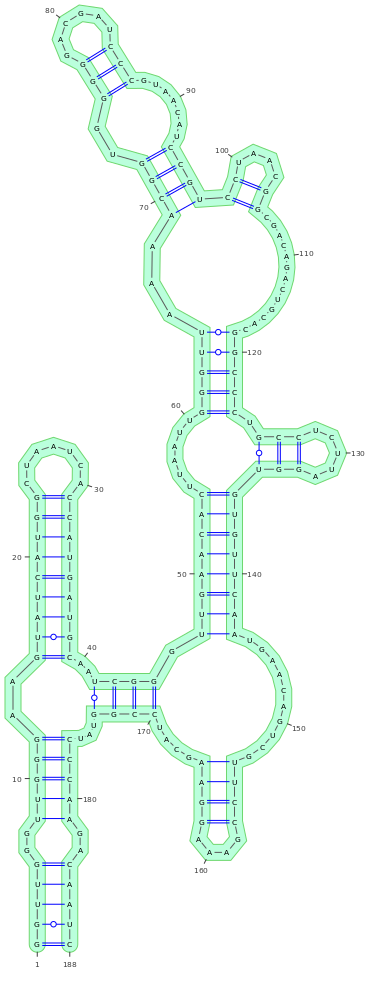
\includegraphics[scale=\MyScale]{graphs/Supp_structures/native_structure}&
 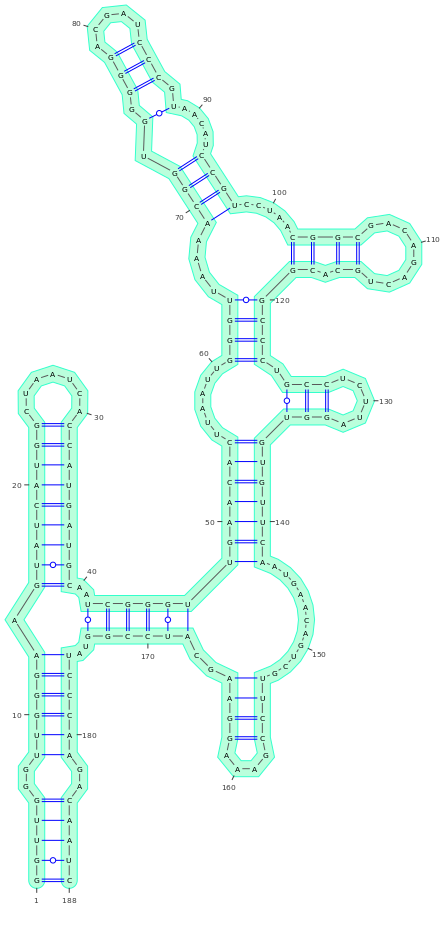
\includegraphics[scale=\MyScale]{graphs/Supp_structures/1M7ILU_NMIAMg}& 
 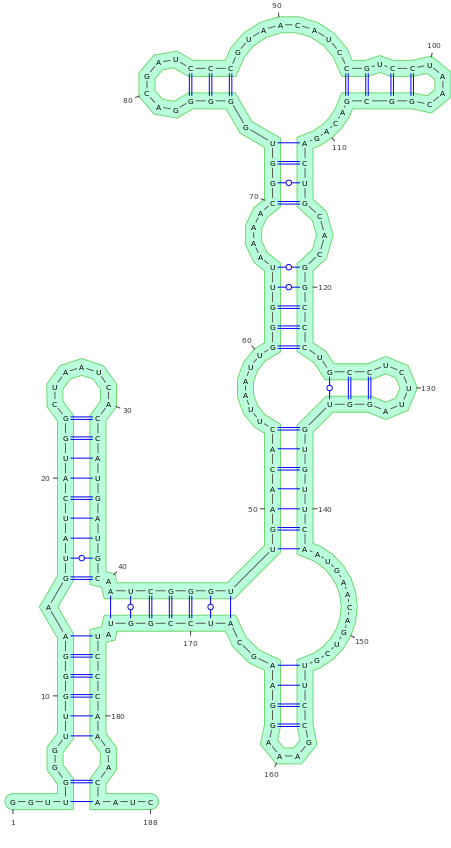
\includegraphics[scale=\MyScale]{graphs/Supp_structures/1M7ILUMg_1M7ILU3Mg}\\
Native&\OneMSevILU&\OneMSevILUMg\\ 
structure &+ \NMIAMg&+ \OneMSevILUThreeMg\\[2em]
 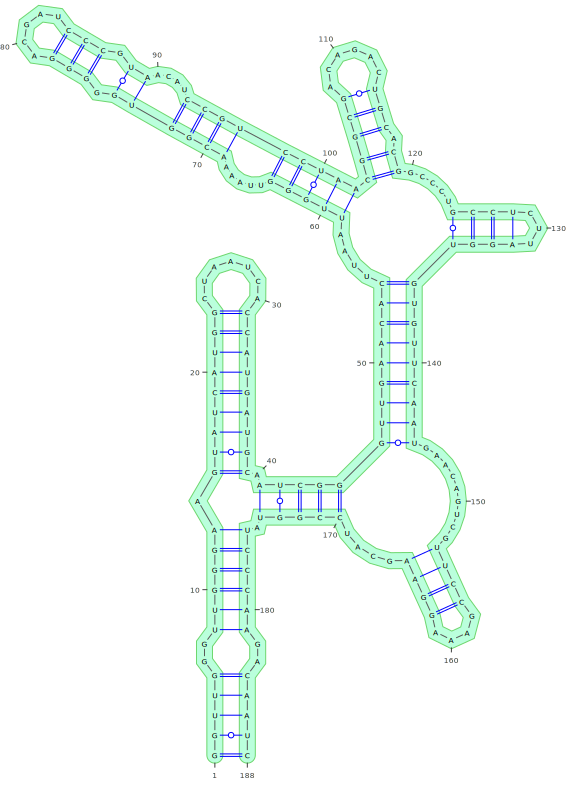
\includegraphics[scale=\MyScale]{graphs/Supp_structures/1M7MgCE_NMIAMgCE}
 &
 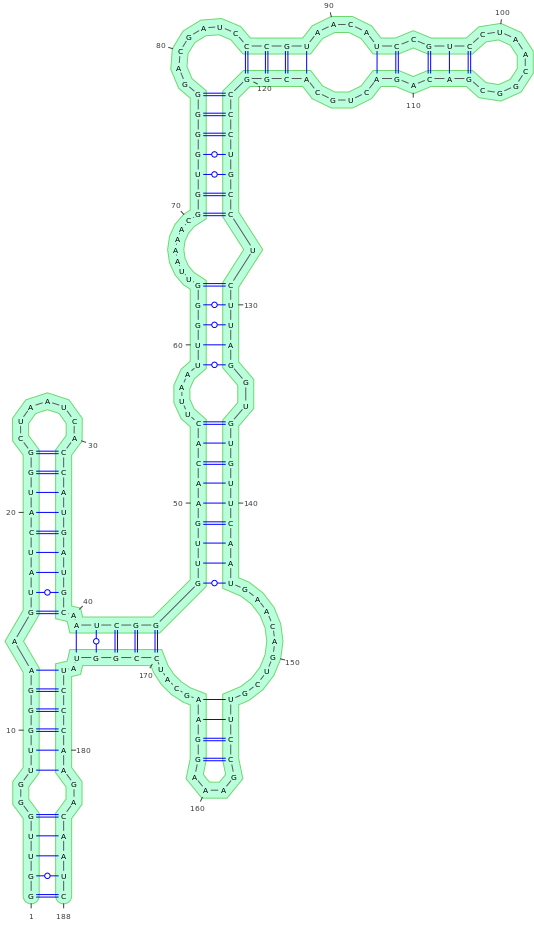
\includegraphics[scale=\MyScale]{graphs/Supp_structures/1M7CE_NMIACE}
 & 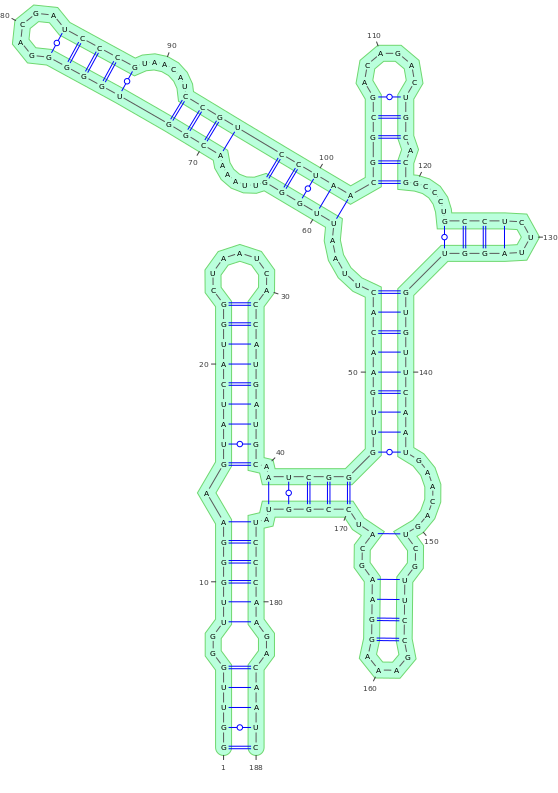
\includegraphics[scale=\MyScale]{graphs/Supp_structures/NaiMg_CMCTMg}\\
\OneMSevMgCE& \OneMSevCE &\NAIMg\\
+ \NMIAMgCE&+ \NMIACE &+ \CMCTMg\\
\end{tabular}
\end{adjustbox}\\}

\caption{Predicted structures with conditions belonging to the same cluster}

\end{figure}



\begin{table}[H]
\newcommand{\MA}[1]{\multicolumn{1}{c}{\Acc{#1}}}
\newcommand{\Acc}[1]{{\bfseries #1}}
\begin{adjustbox}{max width=\textwidth,max totalheight=\textheight,keepaspectratio}
\begin{tabular}{lHHHHHHHHHHHHHHHHH}
	\toprule
	                              & \multicolumn{1}{l}{Mono} & \MA{1} & \MA{2} & \MA{3} & \MA{4} & \MA{5} & \MA{6} & \MA{7} & \MA{8} & \MA{9} & \MA{10} & \MA{11} & \MA{12} & \MA{13} & \MA{14} & \MA{15} & \MA{16} \\ \midrule
	%Mono                         &                          & 0.85   & 0.84   & 0.81   & 0.8    & 0.74   & 0.73   & 0.73   & 0.71   & 0.7    & 0.7     & 0.64    & 0.63    & 0.61    & 0.6     & 0.6     & 0.6     \\
	\Acc{1} -- \OneMSevILUMg      & 0.85                     & 0.85   & 0.84   & 0.8    & 0.82   & 0.82   & 0.82   & 0.75   & 0.79   & 0.78   & 0.79    & 0.79    & 0.85    & 0.61    & 0.79    & 0.79    & 0.85    \\
	\Acc{2} -- \OneMSevILU        & 0.84                     &        & 0.84   & 0.82   & 0.82   & 0.7    & 0.83   & 0.72   & 0.82   & 0.85   & 0.83    & 0.84    & 0.84    & 0.84    & 0.6     & 0.84    & 0.6     \\
	\Acc{3} -- \NMIAMg            & 0.81                     &        &        & 0.81   & 0.8    & 0.74   & 0.82   & 0.82   & 0.81   & 0.81   & 0.79    & 0.8     & 0.8     & 0.61    & 0.81    & 0.81    & 0.6     \\
	\Acc{4} -- \NMIA              & 0.8                      &        &        &        & 0.8    & 0.74   & 0.73   & 0.81   & 0.78   & 0.7    & 0.79    & 0.63    & 0.72    & 0.61    & 0.7     & 0.7     & 0.59    \\
	\Acc{5} -- \OneMSevILUThreeMg & 0.74                     &        &        &        &        & 0.74   & 0.74   & 0.7    & 0.74   & 0.74   & 0.7     & 0.63    & 0.74    & 0.74    & 0.74    & 0.74    & 0.74    \\
	\Acc{6} -- \NMIAMgCE          & 0.73                     &        &        &        &        &        & 0.73   & 0.73   & 0.73   & 0.73   & 0.73    & 0.61    & 0.73    & 0.61    & 0.73    & 0.73    & 0.6     \\
	\Acc{7} -- \NAIMg             & 0.73                     &        &        &        &        &        &        & 0.73   & 0.72   & 0.7    & 0.73    & 0.64    & 0.68    & 0.61    & 0.73    & 0.73    & 0.59    \\
	\Acc{8} -- \BzCNMg            & 0.71                     &        &        &        &        &        &        &        & 0.71   & 0.65   & 0.73    & 0.63    & 0.72    & 0.6     & 0.61    & 0.6     & 0.59    \\
	\Acc{9} -- \OneMSevMgCE       & 0.7                      &        &        &        &        &        &        &        &        & 0.7    & 0.7     & 0.7     & 0.7     & 0.61    & 0.61    & 0.6     & 0.6     \\
	\Acc{10} -- \CMCTMg           & 0.7                      &        &        &        &        &        &        &        &        &        & 0.7     & 0.63    & 0.74    & 0.61    & 0.6     & 0.6     & 0.6     \\
	\Acc{11} -- \OneMSevILUThree  & 0.64                     &        &        &        &        &        &        &        &        &        &         & 0.64    & 0.62    & 0.62    & 0.65    & 0.65    & 0.59    \\
	\Acc{12} -- \DMSMg            & 0.63                     &        &        &        &        &        &        &        &        &        &         &         & 0.63    & 0.61    & 0.6     & 0.6     & 0.6     \\
	\Acc{13} -- \NMIACE           & 0.61                     &        &        &        &        &        &        &        &        &        &         &         &         & 0.61    & 0.62    & 0.6     & 0.6     \\
	\Acc{14} -- \OneMSevCE        & 0.6                      &        &        &        &        &        &        &        &        &        &         &         &         &         & 0.6     & 0.61    & 0.59    \\
	\Acc{15} -- \BzCN             & 0.6                      &        &        &        &        &        &        &        &        &        &         &         &         &         &         & 0.6     & 0.6     \\
	\Acc{16} -- \NAICE            & 0.6                      &        &        &        &        &        &        &        &        &        &         &         &         &         &         &         & 0.6     \\ \bottomrule
\end{tabular}
\end{adjustbox}
\caption{MCC of structures prediction with \OurTool{} from any pair of conditions}.
\end{table}


%\begin{table}
%\begin{center}
%\begin{tabular}{ll}
%Sample size & MCC\\
%\toprule
%
%100 & 0.55 \\
%500 & 0.55  \\
%1000 &  0.81\\
%2000 & 	0.55  \\
%3000 &  0.77 \\
%5000 & 	0.55  \\ 
%10000& 0.8 \\
%\end{tabular}
%\end {center}
%\caption{ MCC of predicted structures in absence of probig data when varyingthe sample size }
%\end{table}

\begin{figure}[H]
%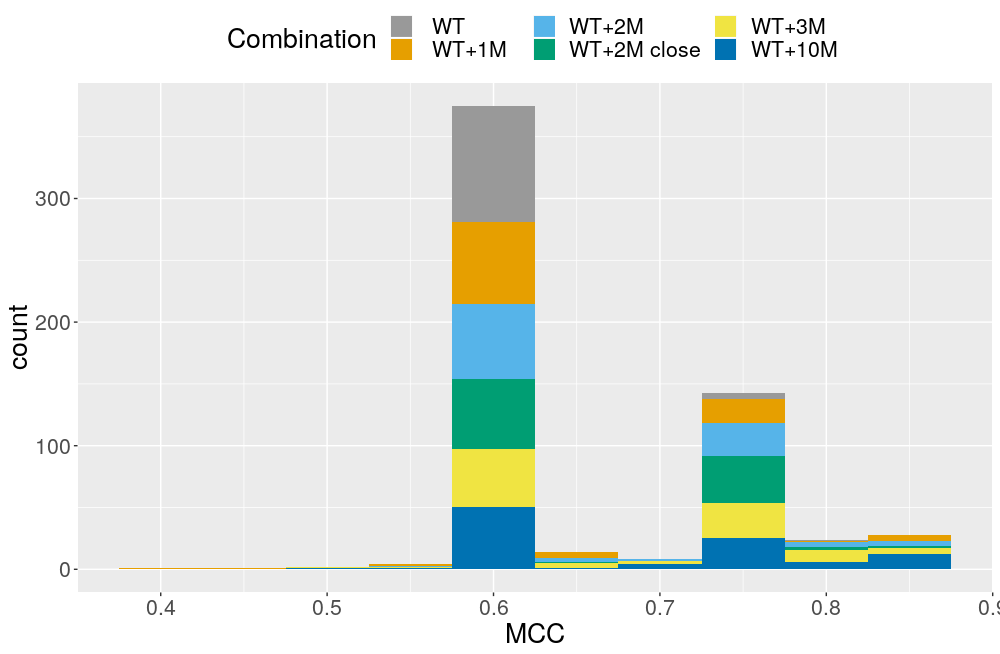
\includegraphics[width=\linewidth]{graphs/histog}
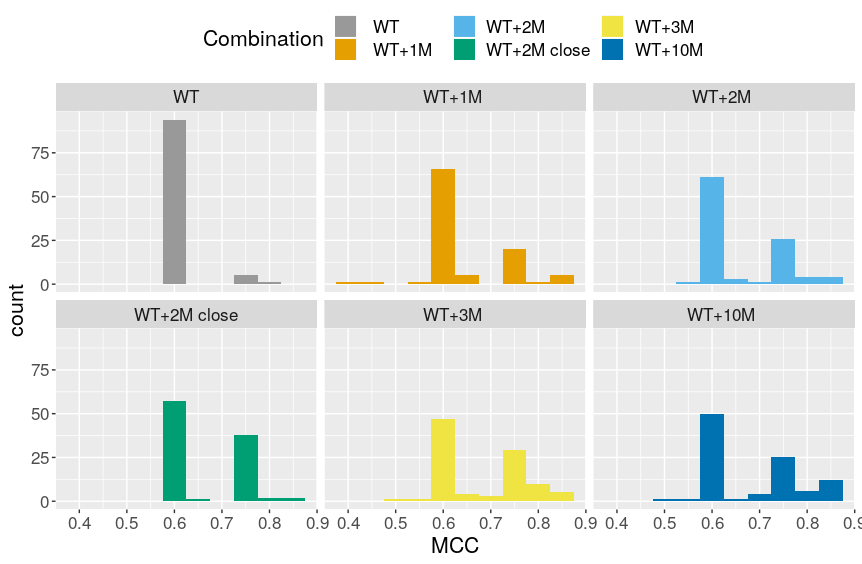
\includegraphics[width=\linewidth]{graphs/histog1}
\caption{Distribution of MCC values over 100 runs from Mutate-and-Map data}
\end{figure}


%\bibliographystyle{bioinformatics}
\bibliographystyle{nar}
%\bibliographystyle{natbib}%compa
\bibliography{biblio}

\end{document}
